\chapter{Diagonalización de Endomorfismos}

\section{Introducción}
\subsection{Espacios Vectoriales}

\begin{notacion}
$V^n(\bb{K})$ representa el espacio vectorial de dimensión $n$ sobre el cuerpo $\bb{K}$ ($\bb{R}$ o $\bb{C}$).
\end{notacion}

\begin{ejemplo} Ejemplos de espacios vectoriales.
\begin{enumerate}
    \item $\bb{K}^n = \left\{ (x_1, \dots , x_n) | x_i \in \bb{K}, i=1, \dots, n \right\}$

    \item $\bb{K}_n[x] = $ \{polinomios con coeficientes en $\bb{K}$ y grado $\leq n\} $

    \item $\mathcal{M}_n(\bb{K}) = $ Matrices cuadradas de orden $n$ y coeficientes en $\bb{K}$.
\end{enumerate}
\end{ejemplo}


\begin{definicion}[Bases]
    La base $\mathcal{B}=\{e_1, \dots, e_n\}$ es un conjunto ``ordenado'' t.q. $\forall v \in V, \; v$ es una combinación lineal de los $e_i$.
    $$v = x_1e_1 + x_2e_2 + \dots + x_ne_n$$
    donde los escalares $x_i$ son únicos.
    $\displaystyle x =
        \left( \begin{array}{c}
             x_1    \\
             \vdots \\
             x_n
        \end{array}\right)$
    son las coordenadas de $v$ respecto de $\mathcal{B}$.
\end{definicion}

\begin{ejemplo} Ejemplos de bases.
\begin{enumerate}
    \item $\mathcal{B}$. $e_1 = (1, 0, \dots, 0)$,\quad $e_2 = (1, 1, 0, \dots, 0)$, \quad \dots

    \item Para $n=2$, $P(x) = a + bx + cx^2$. \quad $\mathcal{B} = \{1, x, x^2\}$\\Coordenadas de $P\equiv (a,b,c)$

    \item $\mathcal{M}_2(\bb{R}) = \left\{
        \left( \begin{array}{cc}
            a & b \\
            c & d
        \end{array}\right)
        | a, b, c, d \in \bb{R} \right\}$

        $e_1 = \left( \begin{array}{cc}
            1 & 0 \\
            0 & 0
        \end{array}\right)$ \quad
        $e_2 = \left( \begin{array}{cc}
            0 & 1 \\
            0 & 0
        \end{array}\right)$ \quad
        $e_3 = \left( \begin{array}{cc}
            0 & 0 \\
            1 & 0
        \end{array}\right)$ \quad
        $e_4 = \left( \begin{array}{cc}
            0 & 0 \\
            0 & 1
        \end{array}\right)$
\end{enumerate}
\end{ejemplo}

\begin{teo} [Cambio de base]
    Sea $\bar{\mathcal{B}}=\{\bar{e_1}, \dots, \bar{e_n}\}$ otra base.
    Sean $\bar{x} = \left( \begin{array}{c}
             \bar{x_1}\\
             \vdots \\
             \bar{x_n}
        \end{array}\right)$ otras coordenadas.
    \begin{equation*}
        x = P\bar{x} \qquad \bar{x} = P^{-1}x
    \end{equation*}
    siendo $P$ la matriz de cambio de base. Sus columna son las coordenadas de $\bar{e_1}, \dots, \bar{e_n}$ respecto de $\mathcal{B}$. $P$ es regular y tiene $n$ filas y $n$ columnas.
\end{teo}

\begin{ejemplo} Ejemplo de cálculo de matriz de cambio de base en el e.v. $\bb{K}_2[x]$.

    Sea $\mathcal{B} = \{1, x, x^2\}$ una base. Sea $\bar{\mathcal{B}} = \{1, x-2, (x-2)^2\}$ otra base.
    
    \begin{equation*}
        P_1(x) = 1 \quad P_2(x) = x-2 \quad P_3(x) = 4-4x+x^2  
    \end{equation*}
    
    \begin{equation*}
        P = \left( \begin{array}{ccc}
         1 & -2 & 4 \\
         0 & 1  & -4 \\
         0 & 0  & 1
        \end{array} \right)
    \end{equation*} 

\end{ejemplo}

\begin{definicion}
    Sea $f:V^n(\bb{K}) \to W^m(\bb{K})$. $f$ es una aplicación lineal si:
    \begin{enumerate}
        \item $f(u+v) = f(u) + f(v)$
        \item $f(du) = df(u)$
    \end{enumerate}
\end{definicion}
\begin{ejercicio*}
    Sea $f:\bb{R}_2[x] \to \bb{R}_2[x]$ aplicación dada por $f(P) = P(1)x + P(-1)(x-1)^2$.
    \begin{enumerate}
        \item Estudiar si $f$ es lineal.
        \item Calcular $A=M(f; \mathcal{B}_u, \mathcal{B}_u)$\footnote{La primera base es referida al espacio de salida, y la segunda al espacio de llegada.}
    \end{enumerate}
\end{ejercicio*}

\section{Valores y vectores propios}
\begin{definicion} [Endomorfismo]
    Sea $V^n(\bb{K})$ y sea $\mathcal{B}$ una base.
    Un endomorfismo es una aplicación lineal $f:V\to V$.
\end{definicion}
\begin{definicion} [Núcleo de un endomorfismo]
    \begin{equation*}
        Ker(f) = \{v\in V | f(v) = 0\}
    \end{equation*}
\end{definicion}
\begin{definicion} [Imagen de un endomorfismo]
    \begin{equation*}
        Im(f) = \{f(v)| v\in V\}
    \end{equation*}
\end{definicion}
\begin{teo}
    \begin{equation*}
        dim_\bb{K}(V) = dim_\bb{K}(Ker(f)) + dim_\bb{K}(Im(f))
    \end{equation*}
\end{teo}

\begin{definicion}
    Dos matrices $A, B\in \mathcal{M}_n(\bb{K})$ son semejantes ($A\sim B$) si $A$ y $B$ representan el mismo endomorfismo pero en bases distintas. Equivalentemente,
    \begin{equation*}
        A \sim B \Longleftrightarrow \exists P \text{ regular t.q. } B = P^{-1}AP
    \end{equation*}
\end{definicion}
\begin{observacion}
$\sim$ es una relación de equivalencia
\end{observacion}
\begin{lema}
    \begin{equation*}
        A \sim B \Longrightarrow \left\{
        \begin{array}{c}
             rg(A) = rg(B) \\
             det(A) = det(B) \\
             tr(A) = tr(B)
        \end{array} \right.
    \end{equation*}
\end{lema}

\begin{ejemplo} Ejemplos de matrices semejantes.
    \begin{enumerate}
        \item La aplicación identidad
        \begin{align*}
            Id:\; V & \longrightarrow V \\
                v & \longmapsto v
        \end{align*}
        
        Si $a \in \bb{K} \Longrightarrow aI$ solo es semejante a ella misma.

        \item
        Sea $A = \left( \begin{array}{cc}
            0&0  \\
            1&1 
        \end{array}\right)$ y 
        $B = \left( \begin{array}{cc}
            0&0  \\
            1&0 
        \end{array}\right)$.
        ¿Son semejantes?

        \begin{itemize}
            \item $AA=A \Longrightarrow f \circ f = f$
            \item $BB=B \Longrightarrow f \circ f = f_0$
        \end{itemize}
        Por tanto, $f=f_0$. Pero $Im(f_0)={0}$, y $rg(A)=rg(B)=1=Dim(f)$. Por tanto, llegamos a una contradicción y vemos que $A\nsim B$.
    \end{enumerate}
\end{ejemplo}

\begin{definicion}[Polinomio característico] Sea $A\in\mathcal{M}_n(\bb{K})$ y sea $P_A(\lambda) \in \bb{K}[\lambda] $  definido como:
    \begin{equation*}
        P_A(\lambda) = det(A-\lambda I)
    \end{equation*}

    $P_A(\lambda)\in \bb{K}[\lambda]$ es un polinomio en la indeterminada $\lambda$, con coeficientes en $\bb{K}$ y de grado $n$.
    \begin{equation*}\begin{split}
        P_A(\lambda) & = det(A-\lambda I) \\
        & = (a_{11}-\lambda)(a_{22}-\lambda)\dots(a_{nn}-\lambda) + \dots \\
        & = (-1)^n\lambda ^n + (-1)^{n-1}[a_{11} + a_{22} + \dots + a_{nn}]\lambda ^{n-1} + \dots\\
        & = (-1)^n\lambda ^n + (-1)^{n-1}tr(A)\lambda ^{n-1} + \dots + det(A)
    \end{split}\end{equation*}
\end{definicion}

\begin{definicion}[Valores propios]
    Sea $A\in\mathcal{M}_n(\bb{K})$. Los valores propios de $A$ son las raíces de $P_A(\lambda)$ y hay como máximo $n$ raíces.
\end{definicion}

\begin{observacion}
    Si la matriz es triangular, los valores propios son los elementos de la diagonal principal.
\end{observacion}

\begin{prop}
    Dos matrices semejantes tienen el mismo polinomio característico.\\
    Sean $A,B\in\mathcal{M}_n(\bb{K})$
    \begin{equation*}
        A \sim B \Longrightarrow P_A(\lambda) = P_B(\lambda)
    \end{equation*}
\end{prop}
\begin{proof}
    \begin{equation*}\begin{split}
        P_B(\lambda) & = det(B-\lambda I) = det(P^{-1}AP - \lambda P^{-1}IP)\\
        & = det(P^{-1}[A-\lambda I]P) = det(A-\lambda I)\\ & = P_A(\lambda)
    \end{split}\end{equation*}
\end{proof}
\begin{ejercicio*} Demostrar lo siguiente:
    \begin{equation*}
        P_A(\lambda) = P_B(\lambda) \nRightarrow A \sim B 
    \end{equation*}

    Sea la matriz $A \in \mathcal{M}_2(\bb{R})$.
    \begin{equation*}
        A = \left(\begin{array}{cc}
            a & b \\
            c & d
        \end{array} \right)
    \end{equation*}
    Calculamos en primer lugar el polinomio caracterísico de $A$.
    \begin{equation*}\begin{split}
        P_A(\lambda) & = det(A-\lambda I)
        = \left| \begin{array}{cc}
            a-\lambda & b \\
            c & d-\lambda
        \end{array} \right|
        = (a-\lambda)(d-\lambda) - bc \\
        & = \lambda ^2 - (a+d)\lambda + ad -bc
    \end{split}\end{equation*}

    Para demostrar lo pedido, se busca un contraejemplo. Sean Las matrices $B,C \in \mathcal{M}_2(\bb{R})$.
    \begin{equation*}\begin{split}
        B = \left(\begin{array}{cc}
            1 & 0 \\
            0 & 1
        \end{array} \right)
        \quad & \quad
        C = \left(\begin{array}{cc}
            1 & 1 \\
            0 & 1
        \end{array} \right)
    \end{split}\end{equation*}
    El polinomio característico de ambas es:
    \begin{equation*}
        P_B(\lambda) = P_C(\lambda) = \lambda ^2 - 2\lambda + 1 = (\lambda -1)^2
    \end{equation*}
    No obstante, $B$ y $C$ no son semejantes, ya que la primera representa la aplicación Identidad mientras que la segunda no. Por tanto, representan distintos endomorfismos. $\hfill \qed$
\end{ejercicio*}

\begin{teo}
    Sea $V$ un espacio vectorial de dimensión $n$ y sea $f \in End(V)$. Tenemos que la aplicación
    \begin{align*}
        End(V) & \longrightarrow \mathcal{M}_n(\bb{K}) \\
        f & \longmapsto M(f, \mathcal{B})
    \end{align*}
    es un isomorfismo.
\end{teo}

\begin{prop}
    Sean $A,B\in\mathcal{M}_n(\bb{K})$
    \begin{equation*}
        A \sim B \Longleftrightarrow \text{Representan el mismo $f$}
    \end{equation*}
\end{prop}
\begin{definicion}
    El polinomio característico de un endomorfismo $f\in End(V)$ que tiene como matriz asociada $A \in \mathcal{M}_n(\bb{K})$ se define como:
    \begin{equation*}\begin{split}
        P_f(\lambda) & = P_A(\lambda) \\
        & = (-1)^n\lambda ^n + (-1)^{n-1}tr(f)\lambda ^{n-1} + \dots + det(f)
    \end{split}\end{equation*}
\end{definicion}
\begin{observacion}
    Como recuerdo, $|f|=0\Longleftrightarrow \ker(f)\neq \{0\} \Longleftrightarrow \nexists f^{-1} $
\end{observacion}

\begin{ejemplo}
    Sean $A_1, A_2, A_3 \in \mathcal{M}_3(\bb{R})$.
    \begin{equation*}
        A_1 = \left( \begin{array}{ccc}
            1 & 2 & 1 \\
            2 & 0 & 2 \\
            1 & 2 & 1 \\
        \end{array}\right) \qquad
        A_2 = \left( \begin{array}{ccc}
            1 & 0 & 1 \\
            1 & 2 & 3 \\
            1 & 1 & -1 \\
        \end{array}\right) \qquad
        A_3 = \left( \begin{array}{ccc}
            3 & -6 & 6 \\
            0 & 1 & 2 \\
            2 & -6 & 3 \\
        \end{array}\right)
    \end{equation*}
    ¿Son semejantes?
    \begin{itemize}
        \item \underline{Opción 1} $PB=AP$, buscar el valor de $P$ y comprobar que es regular.
        \item \underline{Opción 2} Usando las propiedades de las matrices semejantes.
        \begin{table}[H]
            \centering
            \begin{tabular}{r|ccc|l}
                 & $A_1$ & $A_2$ & $A_3$ & \\ \hline
                 $tr(A)$ & $2$ & $2$ & $7$ & $A_1 \nsim A_3 \quad \land \quad A_2 \nsim A_3$ \\
                 $det(A)$ & $0$ & $-6$ & $\times$ & $A_1 \nsim A_2$\\
                 $P_A(\lambda)$ & $\times$ & $\times$ & $\times$ &
            \end{tabular}
            \caption{Resolución del ejemplo usando la opción 2}
        \end{table}
    \end{itemize}
\end{ejemplo}


\begin{definicion}[Multiplicidad algebraica] Sea el polinomio $P(\lambda)$ y sea $\lambda_0$ una raíz de $P(\lambda)$. Se define la multiplicidad algebraica de $\lambda_0$ como:
    \begin{equation*}
        \max\{k\in \bb{N} \mid (\lambda - \lambda_0)^k \text{ divide a } P(\lambda)\}
    \end{equation*}
    \end{definicion}
    
\begin{teo}[Teorema Fundamental del Álgebra]
Todo polinomio $P(\lambda) \in \bb{C}[\lambda]$ con coeficientes en $\bb{C}$ y de grado $n$ tiene exactamente $n$ raíces complejas contadas con multiplicidad algebraica.

Sean $\lambda_1, \dots, \lambda_k \in \bb{C}$ las raíces complejas y sean $m_1, \dots, m_k \in \bb{N}$ sus multiplicidades. Entonces, el polinomio factoriza como:
$$P(\lambda) = a (\lambda - \lambda_1)^{m_1} \dots (\lambda - \lambda_k)^{m_k}$$
siendo $a\in \bb{C}$ el coeficiente líder del polinomio. Además,
$$grd(P) = n = m_1 + \dots + m_k$$
\end{teo}

\begin{teo}
Sea $P(\lambda) \in \bb{R}[\lambda]$ un polinomio real con coeficientes en $\bb{R}$ y de grado $n$. Sean $\lambda_1, \dots, \lambda_k \in \bb{R}$ las raíces reales y sean $m_1, \dots, m_k \in \bb{N}$ sus multiplicidades algebraicas. Entonces, el polinomio factoriza como:
$$P(\lambda) = (\lambda - \lambda_1)^{m_1} \dots (\lambda - \lambda_k)^{m_k} \cdot Q(\lambda)$$
siendo $Q(\lambda) \in \bb{R}[\lambda]$ un polinomio real sin raíces reales. Además,
$$grd(P) = n \geq m_1 + \dots + m_k$$
\end{teo}
\begin{ejemplo}Ejemplos de polinomios reales con distinto número de raíces.
\begin{itemize}
    \item \underline{$grd(P(\lambda)=2$)} \qquad $P(\lambda)=ax^2+bx+c \qquad a,b,c\in \bb{R}$
    \begin{figure}[H]
        \begin{subfigure}{0.3\linewidth}
            \centering
            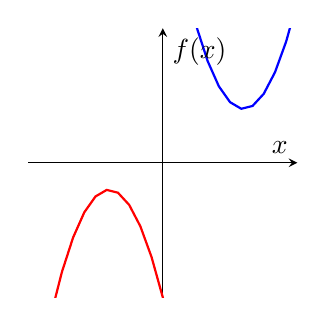
\begin{tikzpicture}
            \begin{axis}[
                xlabel=$x$,
                ylabel=$f(x)$,
                xmin=-5,xmax=5,
                ymin=-5,ymax=5,
                axis lines=middle,
                xtick={0},
                ytick={0},
                width=5cm,
                height=5cm,
                ]
            \addplot[domain=-5:5,blue,thick]{x^2-6*x+11};
            \addplot[domain=-5:5,red,thick]{-x^2-4*x-5};
            \end{axis}
            \end{tikzpicture}
            \caption{Sin raíces}
        \end{subfigure}
        \begin{subfigure}{0.3\linewidth}
            \centering
            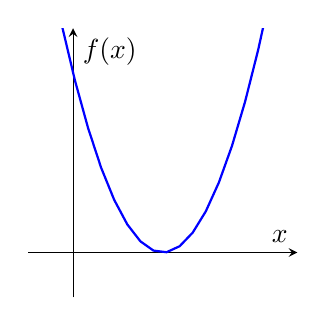
\begin{tikzpicture}
            \begin{axis}[
                xlabel=$x$,
                ylabel=$f(x)$,
                xmin=-1,xmax=5,
                ymin=-1,ymax=5,
                axis lines=middle,
                xtick={0},
                ytick={0},
                width=5cm,
                height=5cm,
                ]
            \addplot[domain=-2:5,blue,thick]{x^2-4*x+4};
            \end{axis}
            \end{tikzpicture}
            \caption{Una raíz}
        \end{subfigure}\begin{subfigure}{0.3\linewidth}
            \centering
            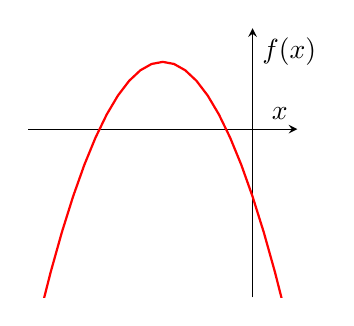
\begin{tikzpicture}
            \begin{axis}[
                xlabel=$x$,
                ylabel=$f(x)$,
                xmin=-5,xmax=1,
                ymin=-5,ymax=3,
                axis lines=middle,
                xtick={0},
                ytick={0},
                width=5cm,
                height=5cm,
                ]
            \addplot[domain=-5:1,red,thick]{-x^2-4*x-2};
            \end{axis}
            \end{tikzpicture}
            \caption{Dos raíces}
        \end{subfigure}
        \caption{Ejemplos de las raíces de un polinomio de grado 2}
    \end{figure}

    \item \underline{$grd(P(\lambda)$ par)} \qquad
    Puede tener o no raíces reales.
    \begin{figure}[H]
        \centering
        \begin{tikzpicture}
        \begin{axis}[
            xlabel=$x$,
            ylabel=$y$,
            xmin=-2,
            xmax=2,
            ymin=-3,
            ymax=3,
            axis lines=middle,
            width=7cm,
            height=5cm,
            samples=90 % número de muestras para la función
        ]
        \addplot[blue,thick,domain=-1:2] {x^8-4*x^7+5*x^3-2*x};
        \end{axis}
        \end{tikzpicture}
        \caption{Ejemplos de las raíces de un polinomio de grado par.}
    \end{figure}

    \item \underline{$grd(P(\lambda)$ impar)} \qquad
    $P(\lambda)$ tiene, al menos, una raíz real\footnote{Los polinomios son funciones continuas en $\bb{R}$, y sus límites en $\pm \infty$ tienen valores consignos opuestos. Por tanto, por el Teorema de Bolzano, tendrá al menos una raíz real.}. Dependerá del polinomio.
    \begin{figure}[H]
        \centering
        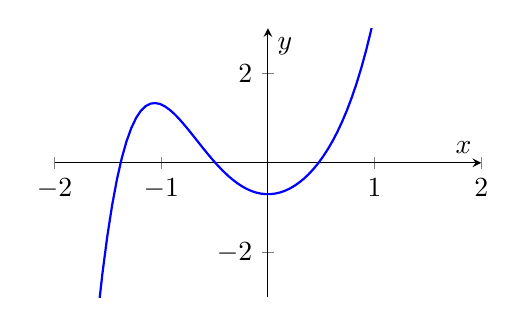
\begin{tikzpicture}
        \begin{axis}[
            xlabel=$x$,
            ylabel=$y$,
            xmin=-2,
            xmax=2,
            ymin=-3,
            ymax=3,
            axis lines=middle,
            width=7cm,
            height=5cm,
            samples=90 % número de muestras para la función
        ]
        \addplot[blue,thick,domain=-2:2] {x^5+3*x^2-0.7};
        \end{axis}
        \end{tikzpicture}
        \caption{Ejemplos de las raíces de un polinomio de grado impar.}
    \end{figure}
\end{itemize}
\end{ejemplo}

\begin{ejercicio*}
    Sean $A,B,C,D \in \mathcal{M}_n(\bb{K}) \mid A \sim B \;\;\land\;\; C \sim D$. Demostrar la falsedad de:
    \begin{enumerate}
        \item $\nRightarrow (A+C) \sim (B+D)$
        \item $\nRightarrow AC \sim BD$
    \end{enumerate}
    
    Sean los valores de $A,B,C,D$ las siguientes matrices:
    \begin{equation*}\begin{array}{cccc}
        A = \left(\begin{array}{cc}
            2 & 4 \\
            2 & 0
        \end{array} \right) &
        B = \left(\begin{array}{cc}
            -2 & 0 \\
            2 & 4
        \end{array} \right) &
        C = \left(\begin{array}{cc}
            1 & 1 \\
            0 & 1
        \end{array} \right) &
        D = \left(\begin{array}{cc}
            3 & 1 \\
            -4 & -1
        \end{array} \right)
    \end{array}\end{equation*}
        
        $A\sim B$, ya que $PB=AP$, con $P = \left(\begin{array}{cc}
            1 & 2 \\
            0 & 1
        \end{array} \right)$.
        
        $C\sim D$, ya que $QD=CQ$, con $Q = \left(\begin{array}{cc}
            1 & 0 \\
            2 & 1
        \end{array} \right)$.

        
    \begin{enumerate}
        \item Los valores de $A+c$ y $B+D$ son:
        \begin{equation*}\begin{array}{cc}
            A+C = \left(\begin{array}{cc}
                3 & 5 \\
                2 & 1
            \end{array} \right) &
            B+D = \left(\begin{array}{cc}
                1 & 1 \\
                -2 & 3
            \end{array} \right)
        \end{array}\end{equation*}
        Como se ve, $(A+c)\nsim (B+D)$, pues $-7=|A+C| \neq |B+D|=5$. $\hfill \qed$

        \item Los valores de $Ac$ y $BD$ son:
        \begin{equation*}\begin{array}{cc}
            AC = \left(\begin{array}{cc}
                2 & 6 \\
                2 & 2
            \end{array} \right) &
            BD = \left(\begin{array}{cc}
                -6 & -2 \\
                -10 & -2
            \end{array} \right)
        \end{array}\end{equation*}
        Como podemos ver, $AC\nsim BD$, ya que $4=tr(AC) \neq tr(BD)=-8$. $\hfill \qed$
    \end{enumerate}
\end{ejercicio*}



\begin{definicion}
    Sea $f\in End(V)$. Los valores propios de un endomorfismo $f$ son las raíces de su polinomio característico.
\end{definicion}


\begin{prop}
    Todo endormorfismo $f\in End(V)$ con dimensión de $V$ impar tendrá al menos un valor propio real.
\end{prop}
\begin{proof}
    Tenemos que su polinomio de característico es de grado 3, y por el Teorema Fundamental del Álgebra tiene al menos una raíz real.
\end{proof}

\begin{definicion} Sea $\lambda_0\in \bb{K}-\{0\}$. EL subespacio propio asociado a $\lambda_0$ se define como:
    \begin{equation*}
        V_{\lambda_0} = \left\{ v\in V \mid f(v)=\lambda_0 v \right\}
    \end{equation*}

    Los elementos $v\in V_{\lambda_0}$ se denominan \emph{vectores propios}.
\end{definicion}

\begin{prop}
    $\lambda_0\in \bb{K}$ es un valor propio $\Longleftrightarrow \exists v \in V-\{0\} \mid f(v)=\lambda_0 v$
\end{prop}
\begin{proof} Sea $\lambda_0 \in \bb{K}$,
    \begin{equation*}
    \begin{split}
         \exists v \in V-\{0\} \mid f(v)=\lambda_0 v & \Longleftrightarrow \exists x \in \bb{K}^n-\{0\} \mid Ax = \lambda_0 x \\
         & \Longleftrightarrow \exists x \in \bb{K}^n-\{0\} \mid (A-\lambda_0 I)x = 0 \\
         & \stackrel{(\ast)}{\Longleftrightarrow} |A-\lambda_0 I|=0 \\
         & \Longleftrightarrow P_A(\lambda_0)=0 \Longleftrightarrow P_f(\lambda_0)=0 \\
         & \Longleftrightarrow \lambda_0 \text{ es una raíz del polinomio característico de } f \text{ o } A\\
         & \Longleftrightarrow \lambda_0 \text{ es un valor propio}.
    \end{split} 
    \end{equation*}

    Donde en $(\ast)$ se ha aplicado que si fuese $|A-\lambda_0 I|\neq 0$, entonces el endomorfismo con matriz asociada $A-\lambda_0 I$ sería biyectivo, por lo que $x$ sería 0.
    
\end{proof}
\begin{observacion}
    $0$ es un valor propio $\Longleftrightarrow \ker(f)\neq \{0\}$
\end{observacion}


\begin{definicion}[Multiplicidad geométrica]
    Se define la multiplicidad geométrica de $\lambda_0$ como la dimensión de $V_{\lambda_0}$.
\end{definicion}

Como consecuencia de dichas definiciones, se cumplen las siguientes propiedades:
\begin{itemize}
    \item $\lambda_0, \lambda_1$ valores propios distintos $\Longrightarrow V_{\lambda_0} \cap V_{\lambda_1} = \{0\}$

    \item Si $\mathcal{B}_1, \dots, \mathcal{B}_n$ son bases de $V_{\lambda_1}, \dots, V_{\lambda_n} \Longrightarrow \mathcal{B}_1 \cup \dots \cup \mathcal{B}_n$ es lin. independiente.

    \item Sea $\lambda_0$ un valor propio y se considera su multiplicidad algebraica $m$ y su multiplicidad geométrica $dim V_{\lambda _0}$. Se cumple:
    $$1 \leq m, \;dim V_{\lambda _0} \leq n$$
\end{itemize}

\begin{lema}
    Sea $\lambda_0$ un valor propio del endomorfismo $f$. Se cumple:
    \begin{equation*}
        \text{Multiplicidad geométrica } \leq \text{ Multiplicidad algebraica}
    \end{equation*}
\end{lema}
\begin{proof}
    Sea $n_0 = dimV_{\lambda_0}$ la multiplicidad geométrica. Sea $m_0$ la multiplicidad algebraica. Se pide demostrar que $n_0 \leq m_0$.
    
    Sea $\mathcal{B}_{\lambda_0} = \{e_1, \dots, e_{n_0}\}$ base de $V_{\lambda_0}$. Ampliamos dicha base a $\mathcal{B}$ base de $V$, $\mathcal{B}=\{e_1, \dots, e_{n_0}, e_{n_0+1}, \dots, e_n\}$. Debido a la elección de las bases, obtenemos que
    \begin{equation*}
        A = M(f;\mathcal{B}) = \left( \begin{array}{c|c}
            \lambda_0 I_{n_0} & B \\ \hline
            0 & C
        \end{array} \right)
    \end{equation*}
    El polinomio característico de $f$ es, por tanto, el siguiente:
    \begin{equation*}
        P_f(\lambda) = \left| \begin{array}{c|c}
            (\lambda_0-\lambda) I_{n_0} & B \\ \hline
            0 & C - \lambda I
        \end{array} \right| = (\lambda_0 - \lambda)^{n_0} Q(\lambda)
    \end{equation*}
    donde se han empleado propiedades de los determinantes de matrices por cajas\footnote{\url{http://wpd.ugr.es/~jperez/wordpress/wp-content/uploads/determinante-por-cajas.pdf}\\Propiedad de las matrices por cajas donde uno de los miembros es $0$.}. Queda demostrado así que $\lambda_0$ divide al polinomio $P_f$ al menos $n_0$ veces, aunque podría dividirlo más veces.
    
    Se demuestra así que $n_0 \leq m_0$.
\end{proof}

\section{Suma Directa}

\begin{definicion}
    Sean $V_1^{n_1}, \dots,V_k^{n_k} \subset V^n$ subespacios vectoriales. Se define la suma de subespacios como:
    $$V_1+\dots +V_k = \left\{ v_1 + \dots v_k \in V \mid v_i \in V_i \right\} \supset V_i$$

    En el cao de que $\mathcal{B}_1,\dots,\mathcal{B}_k$ sean bases de $V_i$,
    $$\mathcal{B}_1\cup \dots \cup \mathcal{B}_k \text{ es un sistema de generadores de la suma.}$$
\end{definicion}
\begin{prop}
    Sean $V_1^{n_1}, \dots,V_k^{n_k} \subset V^n$ subespacios vectoriales.\\
    $V_1+\dots +V_k$ es el menor subespacio que contiene a los $V_i$.
\end{prop}
\begin{prop} Sean $V_1^{n_1}, \dots,V_k^{n_k} \subset V^n$ subespacios vectoriales.
    \begin{equation*}
        \dim (V_1 + \dots + V_k) \leq \dim V_1 + \dots + \dim V_k
    \end{equation*}
\end{prop}

\begin{definicion} Sean $V_1^{n_1}, \dots,V_k^{n_k} \subset V^n$ subespacios vectoriales.
    Decimos que $V_1 + \dots + V_k$ es suma directa, y lo notamos como $$V_1 \oplus \dots \oplus V_k$$ si y solo si:
    \begin{itemize}
        \item $\mathcal{B}_1\cup \dots \cup \mathcal{B}_k$ es base de la suma.

        \item $\dim (V_1 + \dots + V_k) = \dim V_1 + \dots + \dim V_k$

        \item Si $v_i\in V_i \quad i=1,\dots,n \mid v_1+\dots + v_k = 0 \Longrightarrow v_1=v_2=\dots=0$
    \end{itemize}
\end{definicion}

\begin{teo}
    Si $f\in End(V^n(\bb{K}))$ con $\lambda_1, \dots, \lambda_k$ valores propios distintos, entonces $V_{\lambda_1}+\dots + V_{\lambda_k}$ es suma directa.
\end{teo}
\begin{proof}
    Se demuestra por inducción sobre $k$.
    \begin{itemize}
        \item \underline{Para $k=1$} Es trivial.
        \item \underline{Para $k=2$}\\
        Sabemos que $V_{\lambda_1}\cap V_{\lambda_2}=\{0\} \Longrightarrow V_{\lambda_1} \oplus V_{\lambda_2}$ es suma directa de $V_{\lambda_1}$ y $V_{\lambda_1}$.

        \item \underline{Supuesto cierto para $k-1$, comprobemos para $k$}\\
        Sean $v_i \in V_{\lambda_i}\quad i=1, \dots, k$ t.q.
        \begin{equation} \label{Teo14.Ec1}
            v_1 + \dots + v_k = 0
        \end{equation}
        Aplico $f$ y obtengo 
        \begin{equation} \label{Teo14.Ec2}
            \lambda_1v_1 + \dots + \lambda_kv_k = 0
        \end{equation}
        Multiplico la ecuación \ref{Teo14.Ec1} por $\lambda_1$ y obtengo 
        \begin{equation} \label{Teo14.Ec3}
            \lambda_1v_1 + \dots + \lambda_1v_k = 0
        \end{equation}

        Restando las ecuaciones \ref{Teo14.Ec2} y \ref{Teo14.Ec3},
        \begin{equation*}
            (\lambda_2-\lambda_1)v_2 + \dots + (\lambda_k-\lambda_1) = 0
        \end{equation*}

        Como los valores propios son distintos, $\lambda_i-\lambda_1 \neq 0 \quad i=2,\dots,k$. Usando la hipótesis de inducción, $v_2 = \dots = v_k = 0 \Longrightarrow v_1 = 0$, quedando así también demostrado para $k$.
    \end{itemize}
\end{proof}


\section{Diagonalización}

\begin{definicion}
    Decimos que $f\in End(V)$ es diagonalizable si tiene una base de vectores propios.
\end{definicion}

\begin{definicion}
    Decimos que la matriz $A\in \mathcal{M}_n(\bb{K})$ es diagonalizable si $A$ es semejante a una matriz diagonal.
    \begin{equation*}\begin{split}
        A \text{ diagonalizable} & \Longleftrightarrow \exists D \in \mathcal{M}_n(\bb{K}) \mid A \sim D\\
        & \Longleftrightarrow \exists P \in \mathcal{M}_n(\bb{K}) \text{ regular} \mid P^{-1}AP=D, \text{ con D diagonal}.
    \end{split}\end{equation*}
\end{definicion}


\begin{teo}[Teorema fundamental de la diagonalización]
    Sea $f\in End(V(\bb{K}))$ un endomorfismo. Entonces son equivalentes:
    \begin{enumerate}
        \item $f$ es diagonalizable
        
        \item $P_f(\lambda)$ tiene $n$ raíces en $\bb{K}$ contadas con multiplicidad algebraica y, además, la multiplicidad algebraica $m_i$ coincide con la multiplicidad geométrica $n_i \quad \forall i=1,\dots, k$
        \begin{itemize}
            \item $\displaystyle \sum_{i=1}^k m_i = n$
            \item $n_i = m_i \quad \forall i=1,\dots, k$
        \end{itemize}
    \end{enumerate}
\end{teo}
\begin{proof} Se hace mediante doble implicación:
    \begin{description}
        \item [$\mathbf{1) \Longrightarrow 2)}$] Como $f$ es diagonalizable, $\exists \mathcal{B}$ base de $V$ formada por vectores propios. Es decir, se obtiene $\mathcal{B} = \mathcal{B}_1\cup\dots\cup\mathcal{B}_k$. Por tanto, $V = V_{\lambda_1}\oplus\dots\oplus V_{\lambda_k}$, y por tanto,
        $$\dim V = \dim(V_{\lambda_1}) + \dots + \dim(V_{\lambda_k}) \Longrightarrow n = n_1 + \dots + n_k$$
        Además, como $m_i \leq n_i \;\;\forall i \Longrightarrow n = n_1 + \dots  + n_k \leq m_1 + \dots + m_k \leq n$. Por tanto, forzosamente:
        $$n_i = m_i \;\; \forall i = 1,\dots, k \qquad m_1 + \dots + m_k = n$$
        verificando por tanto las condiciones del enunciado.

        
        \item [$\mathbf{2) \Longrightarrow 1)}$]
        Queremos ver que hay una base $\mathcal{B} $ de $V$ de vectores propios.

        Tomamos $\mathcal{B}_1,\dots,\mathcal{B}_k$ bases en $V_{\lambda_1},\dots,V_{\lambda_k}$. Veamos que $\mathcal{B} = \mathcal{B}_1\cup\dots\cup\mathcal{B}_k$.

        Sabemos que $\mathcal{B}$ es una base de $V_{\lambda_1}\oplus\dots\oplus V_{\lambda_k}$. 

        Usando las condiciones del teorema, $|\mathcal{B}| = n_1 + \dots + n_k = m_1 + \dots + m_k = n$. Por tanto, $V_{\lambda_1}\oplus\dots\oplus V_{\lambda_k} = V$, por lo que hay una base de vectores propios y $f$ es diagonalizable.
    \end{description}
\end{proof}

\begin{coro}
Sea $A\in \mathcal{M}_n{(\bb{K})}$. Si $P_A(\lambda)$ tiene $n$ raíces distintas ($m_i=1 \; \forall i$) $\Longrightarrow A$ es diagonalizable.
\end{coro}

\begin{ejemplo}
    Sea $A\in \mathcal{M}_2(\bb{R})$. Estudiar si es o no diagonalizable y diagonalizarla cuando lo sea.
    \begin{enumerate}
        \item $A = \left( \begin{array}{cc}
            1 & 2 \\
            -1 & 0
        \end{array}\right)$

        Obtenemos su polinomio característico:
        \begin{equation*}
            \begin{split}
                P_A(\lambda) &= \lambda^2 - tr(A)\lambda + det(A) \\
                &= \lambda^2 -\lambda + 2
            \end{split}
        \end{equation*}

        Como $\Delta=1-8<0 \Longrightarrow$ No tiene raíces en $\bb{R}$. Por tanto, no hay valores propios ni vectores propios, por lo que NO es diagonalizable.

        \item $A = \left( \begin{array}{cc}
            1 & 0 \\
            -1 & 2
        \end{array}\right)$
        
       Su polinomio característico es $P_A(\lambda) =\lambda^2 -3\lambda +2$, y sus valores propios son $\{1,2\}$. Por el corolario del teorema fundamental de diagonalización, SÍ es diagonalizable.

       Para diagonalizarla, es necesario encontrar $D,P \in \mathcal{M}_2(\bb{R})$, con $P$ regular y $D$ diagonal, t.q. $P^{-1}AP=D$.

       Calculamos en primer lugar los subespacios propios:
       \begin{equation*}\begin{split}
           V_1 & = \left\{ \left(\begin{array}{c}
                x_1 \\
                x_2 
           \end{array}\right) \in \bb{R}^2 \mid (A-I)\left(\begin{array}{c}
                x_1 \\
                x_2 
           \end{array}\right) = 0 \right\} \\
           & = \left\{ \left(\begin{array}{c}
                x_1 \\
                x_2 
           \end{array}\right) \in \bb{R}^2 \mid \left( \begin{array}{cc}
            0 & 0 \\
            -1 & 1
        \end{array}\right) \left(\begin{array}{c}
                x_1 \\
                x_2 
           \end{array}\right) = 0 \right\} \\
           & = \left\{ \left(\begin{array}{c}
                x_1 \\
                x_2 
           \end{array}\right) \in \bb{R}^2 \mid -x_1+x_2=0 \right\} = \mathcal{L}\left(\left\{ \left(\begin{array}{c}
                1 \\
                1 
           \end{array}\right)\right\}\right)
       \end{split}\end{equation*}
       \begin{equation*}\begin{split}
           V_2 & = \left\{ \left(\begin{array}{c}
                x_1 \\
                x_2 
           \end{array}\right) \in \bb{R}^2 \mid (A-2I)\left(\begin{array}{c}
                x_1 \\
                x_2 
           \end{array}\right) = 0 \right\} \\
           & = \left\{ \left(\begin{array}{c}
                x_1 \\
                x_2 
           \end{array}\right) \in \bb{R}^2 \mid \left( \begin{array}{cc}
            -1 & 0 \\
            -1 & 0
        \end{array}\right) \left(\begin{array}{c}
                x_1 \\
                x_2 
           \end{array}\right) = 0 \right\} \\
           & = \left\{ \left(\begin{array}{c}
                x_1 \\
                x_2 
           \end{array}\right) \in \bb{R}^2 \mid x_1=0 \right\} = \mathcal{L}\left(\left\{ \left(\begin{array}{c}
                0 \\
                1 
           \end{array}\right)\right\}\right)
       \end{split}\end{equation*}

       Por tanto, una base de vectores propios es $\mathcal{B}=\left\{\left(\begin{array}{c}
                1 \\
                1 
           \end{array}\right),\left(\begin{array}{c}
                0 \\
                1 
           \end{array}\right)
       \right\}$.
       
       Por tanto,
       \begin{equation*}
       D\footnote{En la diagonal se colocan los valores propios.}
       =\left(\begin{array}{cc}
           1 & 0 \\
           0 & 2
       \end{array}\right) \qquad
       P\footnote{En las columnas se colocan los vectores de la base de vectores propios.}
        =\left(\begin{array}{cc}
           1 & 0 \\
           1 & 1
       \end{array}\right)
       \end{equation*}

        \item $A = \left( \begin{array}{cc}
            0 & 1 \\
            -1 & 2
        \end{array}\right)$

        Su polinomio característico es $P_A(\lambda) =\lambda^2 -2\lambda +1 = (\lambda-1)^2$, y su valor propios es $\lambda_1=1$ con multiplicidad algebraica $m_1=2$.

        Calculamos el subespacio propio:
       \begin{equation*}\begin{split}
           V_1 & = \left\{ \left(\begin{array}{c}
                x_1 \\
                x_2 
           \end{array}\right) \in \bb{R}^2 \mid (A-I)\left(\begin{array}{c}
                x_1 \\
                x_2 
           \end{array}\right) = 0 \right\} \\
           & = \left\{ \left(\begin{array}{c}
                x_1 \\
                x_2 
           \end{array}\right) \in \bb{R}^2 \mid \left( \begin{array}{cc}
            -1 & 1 \\
            -1 & 1
        \end{array}\right) \left(\begin{array}{c}
                x_1 \\
                x_2 
           \end{array}\right) = 0 \right\} \\
           & = \left\{ \left(\begin{array}{c}
                x_1 \\
                x_2 
           \end{array}\right) \in \bb{R}^2 \mid -x_1+x_2=0 \right\} = \mathcal{L}\left(\left\{ \left(\begin{array}{c}
                1 \\
                1 
           \end{array}\right)\right\}\right)
       \end{split}\end{equation*}
       Por tanto, $n_1 = dim V_1 = 1$. Como $n_1 = 1 \neq 2 = m_1$, por el Teorema Fundamental de la Diagonalización, $A$ NO es diagonalizable.
    \end{enumerate}
\end{ejemplo}


\begin{ejemplo}
   Ejemlos de matrices $A \in \mathcal{M}_2(\bb{K})$ diagonalizables o no con valor propio $a\in \bb{K}$ y multiplicidad algebráica $m_a=2$.
   \begin{itemize}
       \item \underline{Sí es diagonalizable}
       \begin{equation*}
           A = \left( \begin{array}{cc}
               a & 0 \\
               0 & a
           \end{array} \right)
       \end{equation*}

       \item \underline{No es diagonalizable}
       \begin{equation*}
           A = \left( \begin{array}{cc}
               a & 0 \\
               b & a
           \end{array} \right)
       \end{equation*}
       Su polinomio característico es $P_A(\lambda) = \lambda^2 - 2a\lambda + a^2 = (\lambda-a)^2$.
       
       El subespacio propio es $V_a = \{x \in \bb{K}^2 \mid x_2 = 0\}$, por lo que la multiplicidad geométrica es $n_a=1$, por lo que no es diagonalizable.
   \end{itemize}
\end{ejemplo}

\section{Teorema de Cayley-Hamilton}

Es fácil ver que, al igual que trabajamos con $x\in \bb{R}$, se pueden evaluar polinomios en matrices, sabiendo que $A^0 = I$.
$$P(A) = a_mA^m + \dots a_1A + a_0I$$

Al igual que, para $x\in \bb{R}$, tenemos los binomios notables, también se dan para matrices. Al igual que $x^2-1 = (x+1)(x-1)$,$$A^2-I = (A+I)(A-I)$$

\begin{lema}
    Sea $P\in \mathcal{M}_n(\bb{K})$ regular y sea $A\in \mathcal{M}_n(\bb{K})$. Dada $B\in \mathcal{M}_n(\bb{K}) \mid A\sim B$,

    \begin{equation*}
        B^k = (P^{-1}AP)^k = P^{-1}A^kP
    \end{equation*}
\end{lema}
\begin{proof}
    Se demuestra por inducción.\\
    Para $k=2$,
    \begin{equation*}
        B^2 = (P^{-1}AP)^2 = P^{-1}APP^{-1}AP = P^{-1}A^2P
    \end{equation*}
\end{proof}

\begin{coro}
    $$p(P^{-1}AP) = P^{-1}p(A)P$$
\end{coro}

\begin{lema}
    Sea $A\in\mathcal{M}_n(\bb{K})$ dada por:
    \begin{equation*}
        A = \left( \begin{array}{c|c}
            A_1 & A_3 \\ \hline
            0 & A_2
        \end{array} \right)
    \end{equation*}
    con $A_1,\;A_2$ cuadradas. Se comprueba que:
    \begin{equation*}
        A^k = \left( \begin{array}{c|c}
            A_1^k & B_k \\ \hline
            0 & A_2^k
        \end{array} \right)
    \end{equation*}
\end{lema}
\begin{proof}
    Se demuestra por inducción.\\
    Para $k=2$,
    \begin{equation*}
        A^2 = \left( \begin{array}{c|c}
            A_1 & A_3 \\ \hline
            0 & A_2
        \end{array} \right)
        \left( \begin{array}{c|c}
            A_1 & A_3 \\ \hline
            0 & A_2
        \end{array} \right) = 
        \left( \begin{array}{c|c}
            A_1^2 & B \\ \hline
            0 & A_2^2
        \end{array} \right)
    \end{equation*}
\end{proof}

\begin{coro}
    \begin{equation*}
        p(A) = \left( \begin{array}{c|c}
            p(A_1) & C \\ \hline
            0 & p(A_2)
        \end{array} \right)
    \end{equation*}
\end{coro}

\begin{teo} [Teorema de Cayley-Hamilton]

Sea $A\in\mathcal{M}_n(\bb{K})$. \begin{equation*}
    P_A(A) = 0
\end{equation*}
\end{teo}

\begin{proof}
    Puedo suponer $\bb{K}=\bb{C}$, ya que $\bb{R} \subset \bb{C}$. Demostramos el teorema por inducción sobre $n$.

    \begin{itemize}
        \item \underline{Para $n=1$}:\\
        Sea $A=(a)$.Además, $I_1 = (1)$.
        \begin{equation*}
            P_A(A) = |A-AI| = det((a)-(a)) = det(0) = 0
        \end{equation*}

        \item \underline{Supuesto cierto para $n-1$, lo comprobamos para $n$}:\\
        $\exists \lambda_1\in \bb{C}$ valor propio de $A$. Sea $e_1$ un vector propio.
        Amplío $\{e_1\}$ a una base $\mathcal{B}$ de $\bb{C}^n$. $\mathcal{B} = \{e_1, \dots e_k\}$.\\
        $A$ es semejante a $\left(\begin{array}{c|c}
            \lambda_1 & A_3 \\ \hline
            0 & A_2
        \end{array}\right)$. En adelante, denotamos $A=\left(\begin{array}{c|c}
            \lambda_1 & A_3 \\ \hline
            0 & A_2
        \end{array}\right)$, ya que demostrarlo para una matriz semejante es equivalente.
        \begin{equation*}
            P_{A}(\lambda) = det\left(\begin{array}{c|c}
                \lambda_1 - \lambda & A_3 \\ \hline
                0 & A_2 - \lambda I
            \end{array}\right) = (\lambda_1 - \lambda) det(A_2 - \lambda I) = (\lambda_1 - \lambda)P_{A_2}(\lambda)
        \end{equation*}

        Por tanto, evaluando en $\lambda = A$,
        \begin{multline*}
            P_{A}(A) =
            (\lambda_1 I - A)P_{A_2}(A)
            = \left[ \left(\begin{array}{c|c}
                \lambda_1 & 0 \\ \hline
                0 & \lambda_1 I
            \end{array}\right) - \left(\begin{array}{c|c}
                \lambda_1 & A_3 \\ \hline
                0 & A_2
            \end{array}\right)
            \right] \cdot 
            \left(\begin{array}{c|c}
                P_{A_2}(\lambda_1) & D \\ \hline
                0 & P_{A_2}(A_2)
            \end{array}\right) = \\
            = \left(\begin{array}{c|c}
                0 & -A_3 \\ \hline
                0 & \lambda_1 I - A_2
            \end{array}\right)
            \left(\begin{array}{c|c}
                P_{A_2}(\lambda_1) & D \\ \hline
                0 & 0
            \end{array}\right) = 
            \left(\begin{array}{c|c}
                0 & 0 \\ \hline
                0 & 0
            \end{array}\right) = 0
        \end{multline*}
        
        donde se ha aplicado la hipótesis de inducción para saber que $P_{A_2}(A_2) = 0$.\qedhere
    \end{itemize}
\end{proof}

\begin{prop}
    Sea $p(x)\in \bb{K}[x]$, y sea $A\in \mathcal{M}_n(\bb{K})$. Entonces,
    \begin{center}
        $A$ diagonalizable $\Longrightarrow p(A)$ diagonalizable.
    \end{center}
\end{prop}
\begin{observacion}
    Para comprobar que $A\sim B$, a las muy malas y como último recurso, se puede utilizar que:
    $$A\sim B \Longrightarrow A-I \sim B-I$$
\end{observacion}



\section{Ejercicios}
Los ejercicios resueltos del presente tema están disponibles en la sección \ref{sec:EjerciciosTema1}.